\documentclass{article}[18pt]
\usepackage{../../../../../format}
\lhead{CSys}


\begin{document}
\begin{center}
\underline{\huge Boolean Algebra}
\end{center}
\section{Boolean Operations}
There are $2^{2^k}$ possible boolean operations on k inputs
\subsection{XOR}
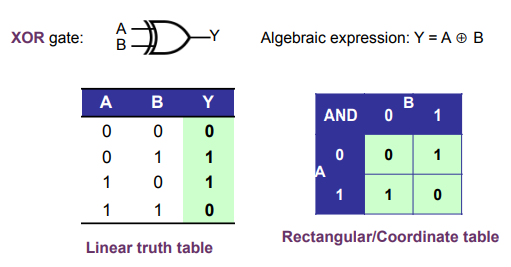
\includegraphics[scale=0.7]{XOR.png}\\
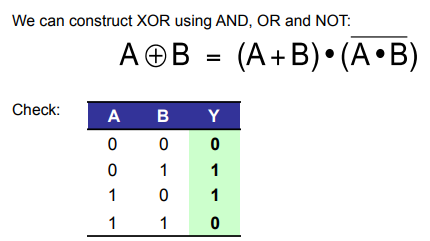
\includegraphics[scale=0.7]{XOR2.png}\\
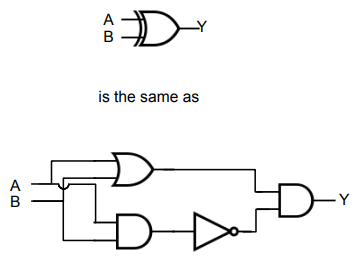
\includegraphics[scale=0.7]{XOR3.png}
\section{Functionally complete sets}
Any logic circuit can be constructed from just the 3 operators:
\begin{itemize}
\item AND, OR, NOT
\item They form a functionally complete set
\item It has been shown that NOR gates alone form a functionally complete set
\end{itemize}
\subsection{NOR Gates}
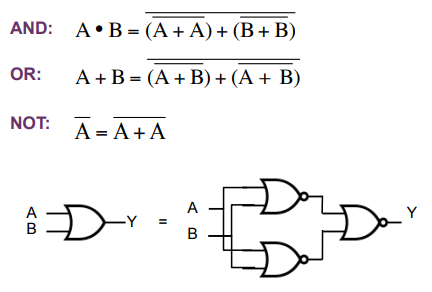
\includegraphics[scale=0.7]{NOR.png}
\subsection{NAND Chips}
NAND gates are easier to make (use less silicon for same performance) than NOR gates, so are often used as universal gates
\section{Digital Design Principles}
Digital design is all about managing the complexity of huge numbers of
interacting elements. Some principles help humans do this:
\begin{itemize}
\item Abstraction: Hiding details when they aren’t important.
\item Discipline: Restricting design choices to make things easier to model, design
and combine. E.g. the logic families and the digital abstraction.
\end{itemize}
The three –y’s:
\begin{itemize}
\item Hierarchy: dividing a system into modules and submodules
\item Modularity: well-defined functions and interfaces for modules
\item Regularity: encouraging uniformity to modules can be swapped or reused.
\end{itemize}
\subsection{Circuits}
A circuit has:
\begin{itemize}
\item one or more discrete valued input terminals
\item one or more discrete valued output terminals
\item a specification of the relationship between inputs and outputs
\item a specification of the delay between inputs changing and outputs - performance specification
responding
\end{itemize}
The circuit is made up of elements and nodes:
\begin{itemize}
\item An \textbf{element} is itself a circuit with inputs, outputs and specs.
\item A \textbf{node} is a wire joining elements, whose voltage conveys a discrete
valued variable.
\end{itemize}
\subsection{Combinatorial Logic}
We wish to design very large circuits to perform functions for us.
Arbitrary circuits can include short circuits and instability, so we restrict what
we allow, firstly to combinational logic (and later sequential logic). 
Combinational logic rules:
\begin{itemize}
\item \textbf{Individual gates} are combinational circuits.
\item  Every circuit \textbf{element} must be a combinational circuit.
\item  Every node is either an input to the circuit or connecting to \textbf{exactly
one output} of a circuit element
\item  The circuit has\textbf{ no cyclic paths} – every path through the circuit
visits any node at most once.
\end{itemize}
\section{Boolean Algebra}
\begin{itemize}
\item  The algebra of 0/1 variables.
\item  Used for specifying the function of a combinational circuit
\item  Used to analyse and simplify the circuits required to give a specified truth
table.
\end{itemize}

Variables are represented by letters, e.g. A, B, C…\\
The complement or inverse of a variable is written with a bar, e.g. A.\\
\\
A variable or its complement is called a literal, e.g. A, $\overline{A}$, B or $\overline{B}$.\\
\\
The AND of several literals is called a \textbf{product} or \textbf{implicant}, e.g. ABC or AC,\\
Products may be written $A\cdot B\cdot C$, ABC, $A\cap B\cap C$ or $A\land B\land C$.\\
A \textbf{minterm} is a product involving all the inputs to a function.\\
\\
The OR of several literals is called a \textbf{sum} or \textbf{implicant}, e.g. A+B+C or A+C,\\
Sums may be written A+B+C, $A\cup B\cup C$ or $A\lor B\lor C$.\\
A \textbf{maxterm} is a sum involving all the inputs to a function.
\subsection{Truth Table to Boolean Equation}
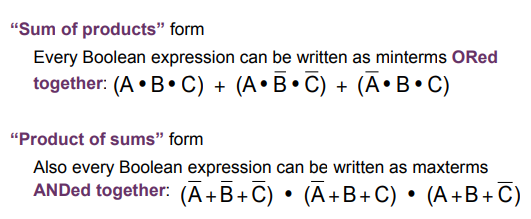
\includegraphics[scale=0.7]{TruthToBool.png}
\subsection{Truth Table to SOP (Sum of Products)}
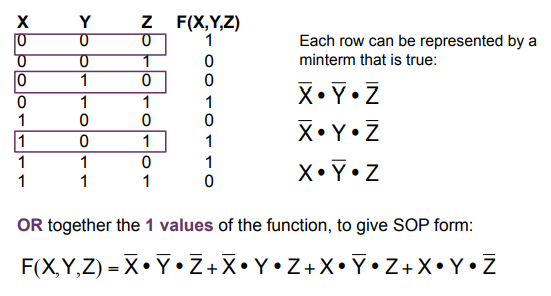
\includegraphics[scale=0.7]{TruthToSOP.png}
\begin{itemize}
	\item The minterms are true only for the combination of inputs
	\item Note that the diagram above has the wrong row highlighted, make modifications myself.
\end{itemize}
\subsection{Example}
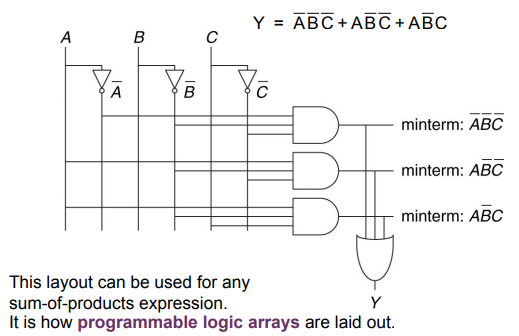
\includegraphics[scale=0.7]{Example.png}\\
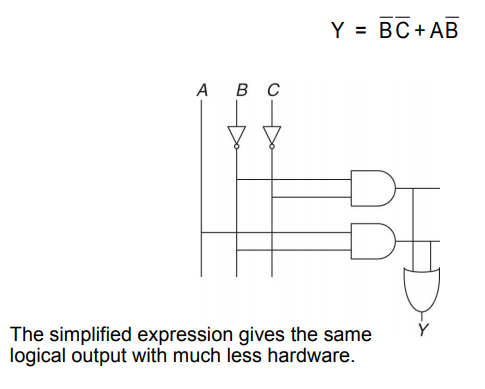
\includegraphics[scale=0.7]{Example2}

\subsection{Truth Table to POS}
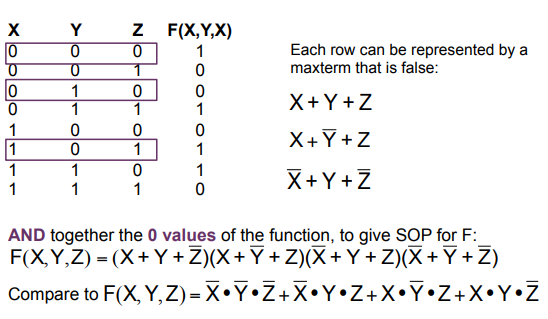
\includegraphics[scale=0.7]{TruthToPOS.png}
\begin{itemize}
	\item These are specified so that the situation does not come up that you are on a 0 row
\end{itemize}
\subsection{Boolean Algebra}
Two equivalent expression for the same logical formula: \\
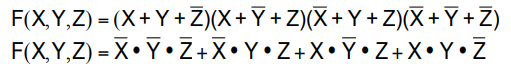
\includegraphics[scale=0.7]{BoolForm.png}\\
Which is simpler?\\
Is there another equivalent expression that is simpler than either?\\
\\
We will use Boolean algebra and Karnaugh maps to produce the simplest
equivalent expression that can then be turned into circuitry
\section{Axioms of Boolean Algebra}
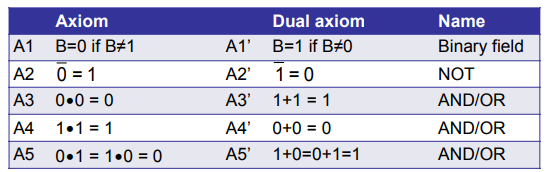
\includegraphics[scale=0.7]{Axioms.png}\\
Axioms cannot be proven – they are defined or assumed.\\
Each axiom has a dual obtained by interchanging AND and OR,
and 0 and 1.
\section{Theorems of several variables}
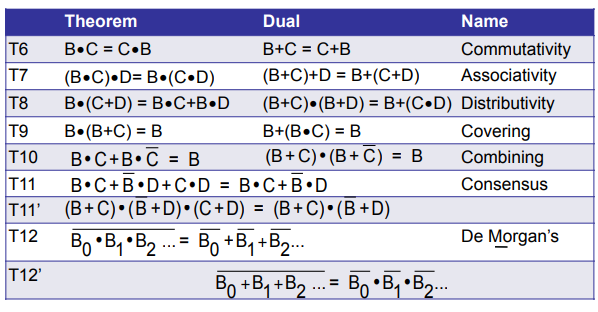
\includegraphics[scale=0.7]{SeveralVar.png}\\
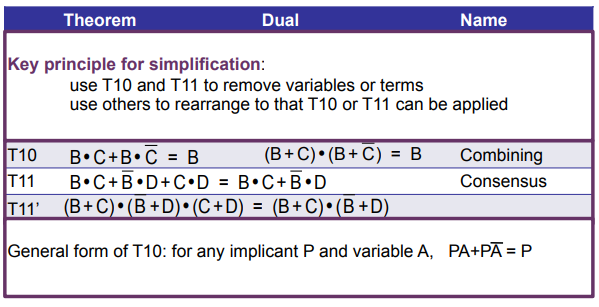
\includegraphics[scale=0.7]{SeveralVar2.png}
\section{De Morgans}
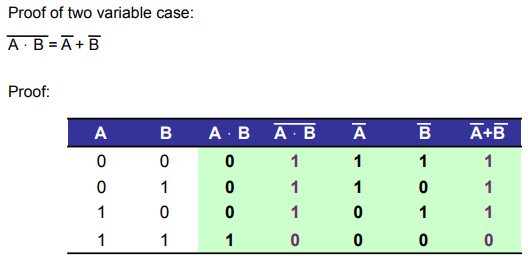
\includegraphics[scale=0.7]{DeMorgan.png}

\end{document}